\documentclass[preview, border=2pt]{standalone}
%\documentclass[varwidth, border=2pt,convert={png,size=1714,density=300}]{standalone}
%\documentclass[varwidth, border=2pt]{standalone}
\usepackage{graphicx}
\usepackage{caption}
\usepackage{subcaption}
\captionsetup[subfigure]{font={scriptsize}, skip=0pt, aboveskip=0cm, belowskip=-10pt, margin=0cm, singlelinecheck=false}
%\captionsetup[subfigure]{labelformat=simple, labelsep=space, justification=raggedright, singlelinecheck=false}
%\renewcommand{\thesubfigure}{(\alph{subfigure})} % Format as (a), (b), (c)

\usepackage{geometry}

\begin{document}

\begin{figure}
     \centering
     \begin{subfigure}[b]{0.24\textwidth}
         \centering         
         \caption{}
         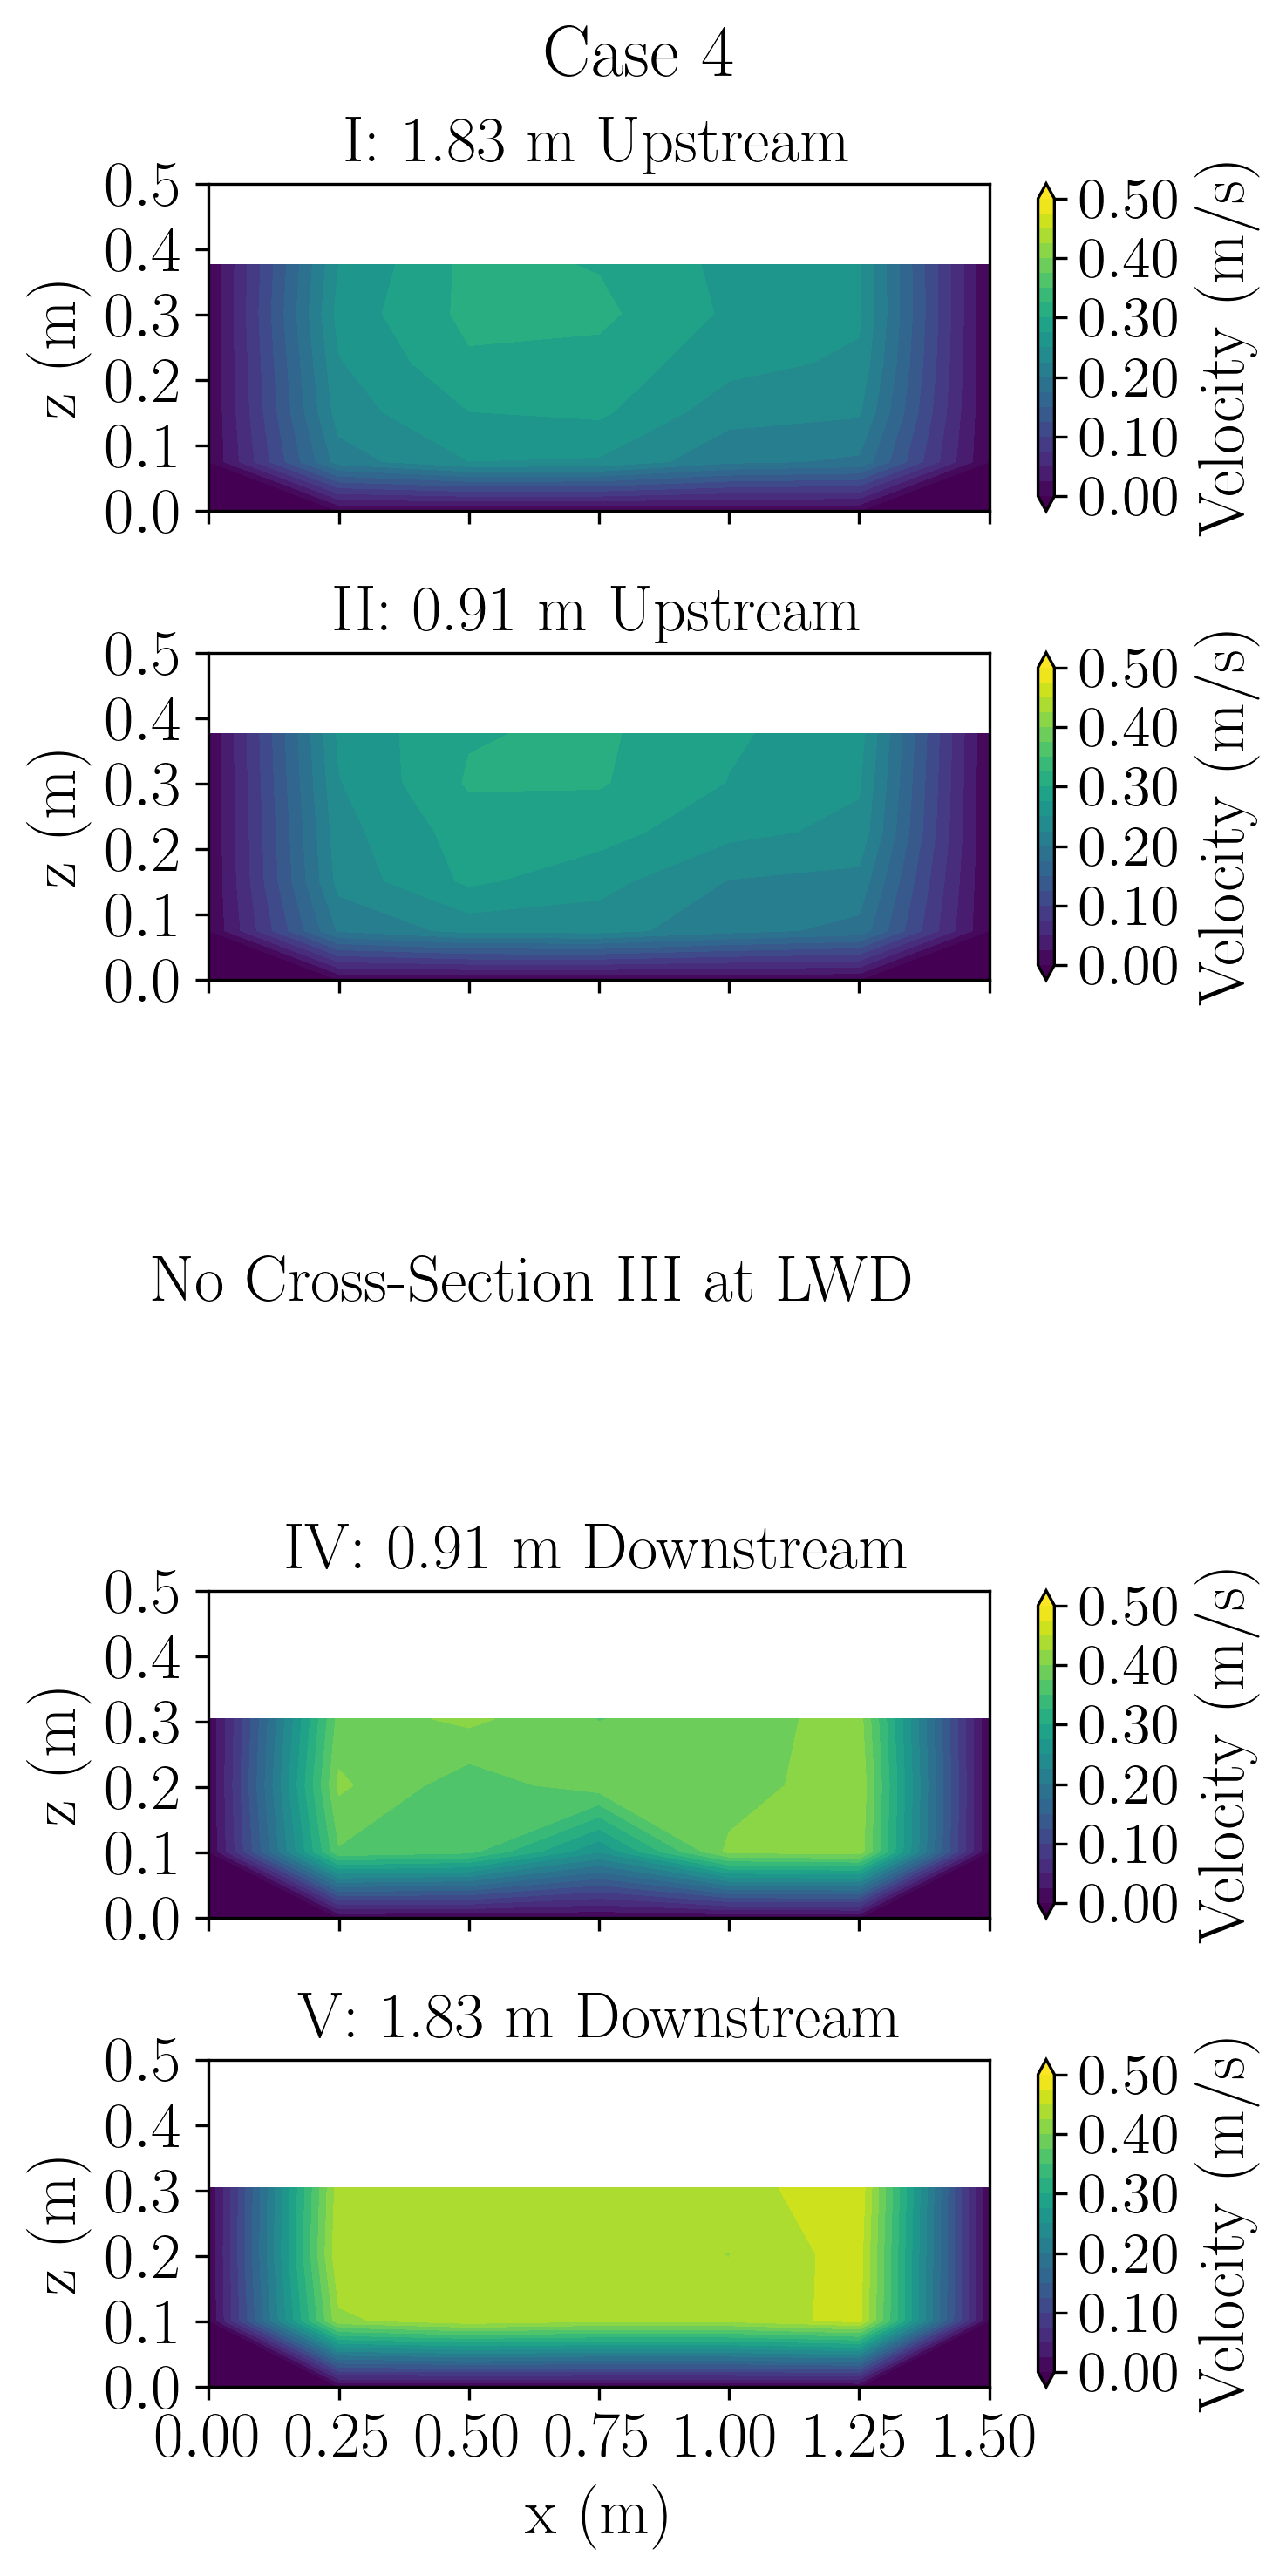
\includegraphics[width=\textwidth]{Case4_velocity_contours.png}         
     \end{subfigure}
     \hfill     
     \begin{subfigure}[b]{0.24\textwidth}
         \centering
         \caption{}
         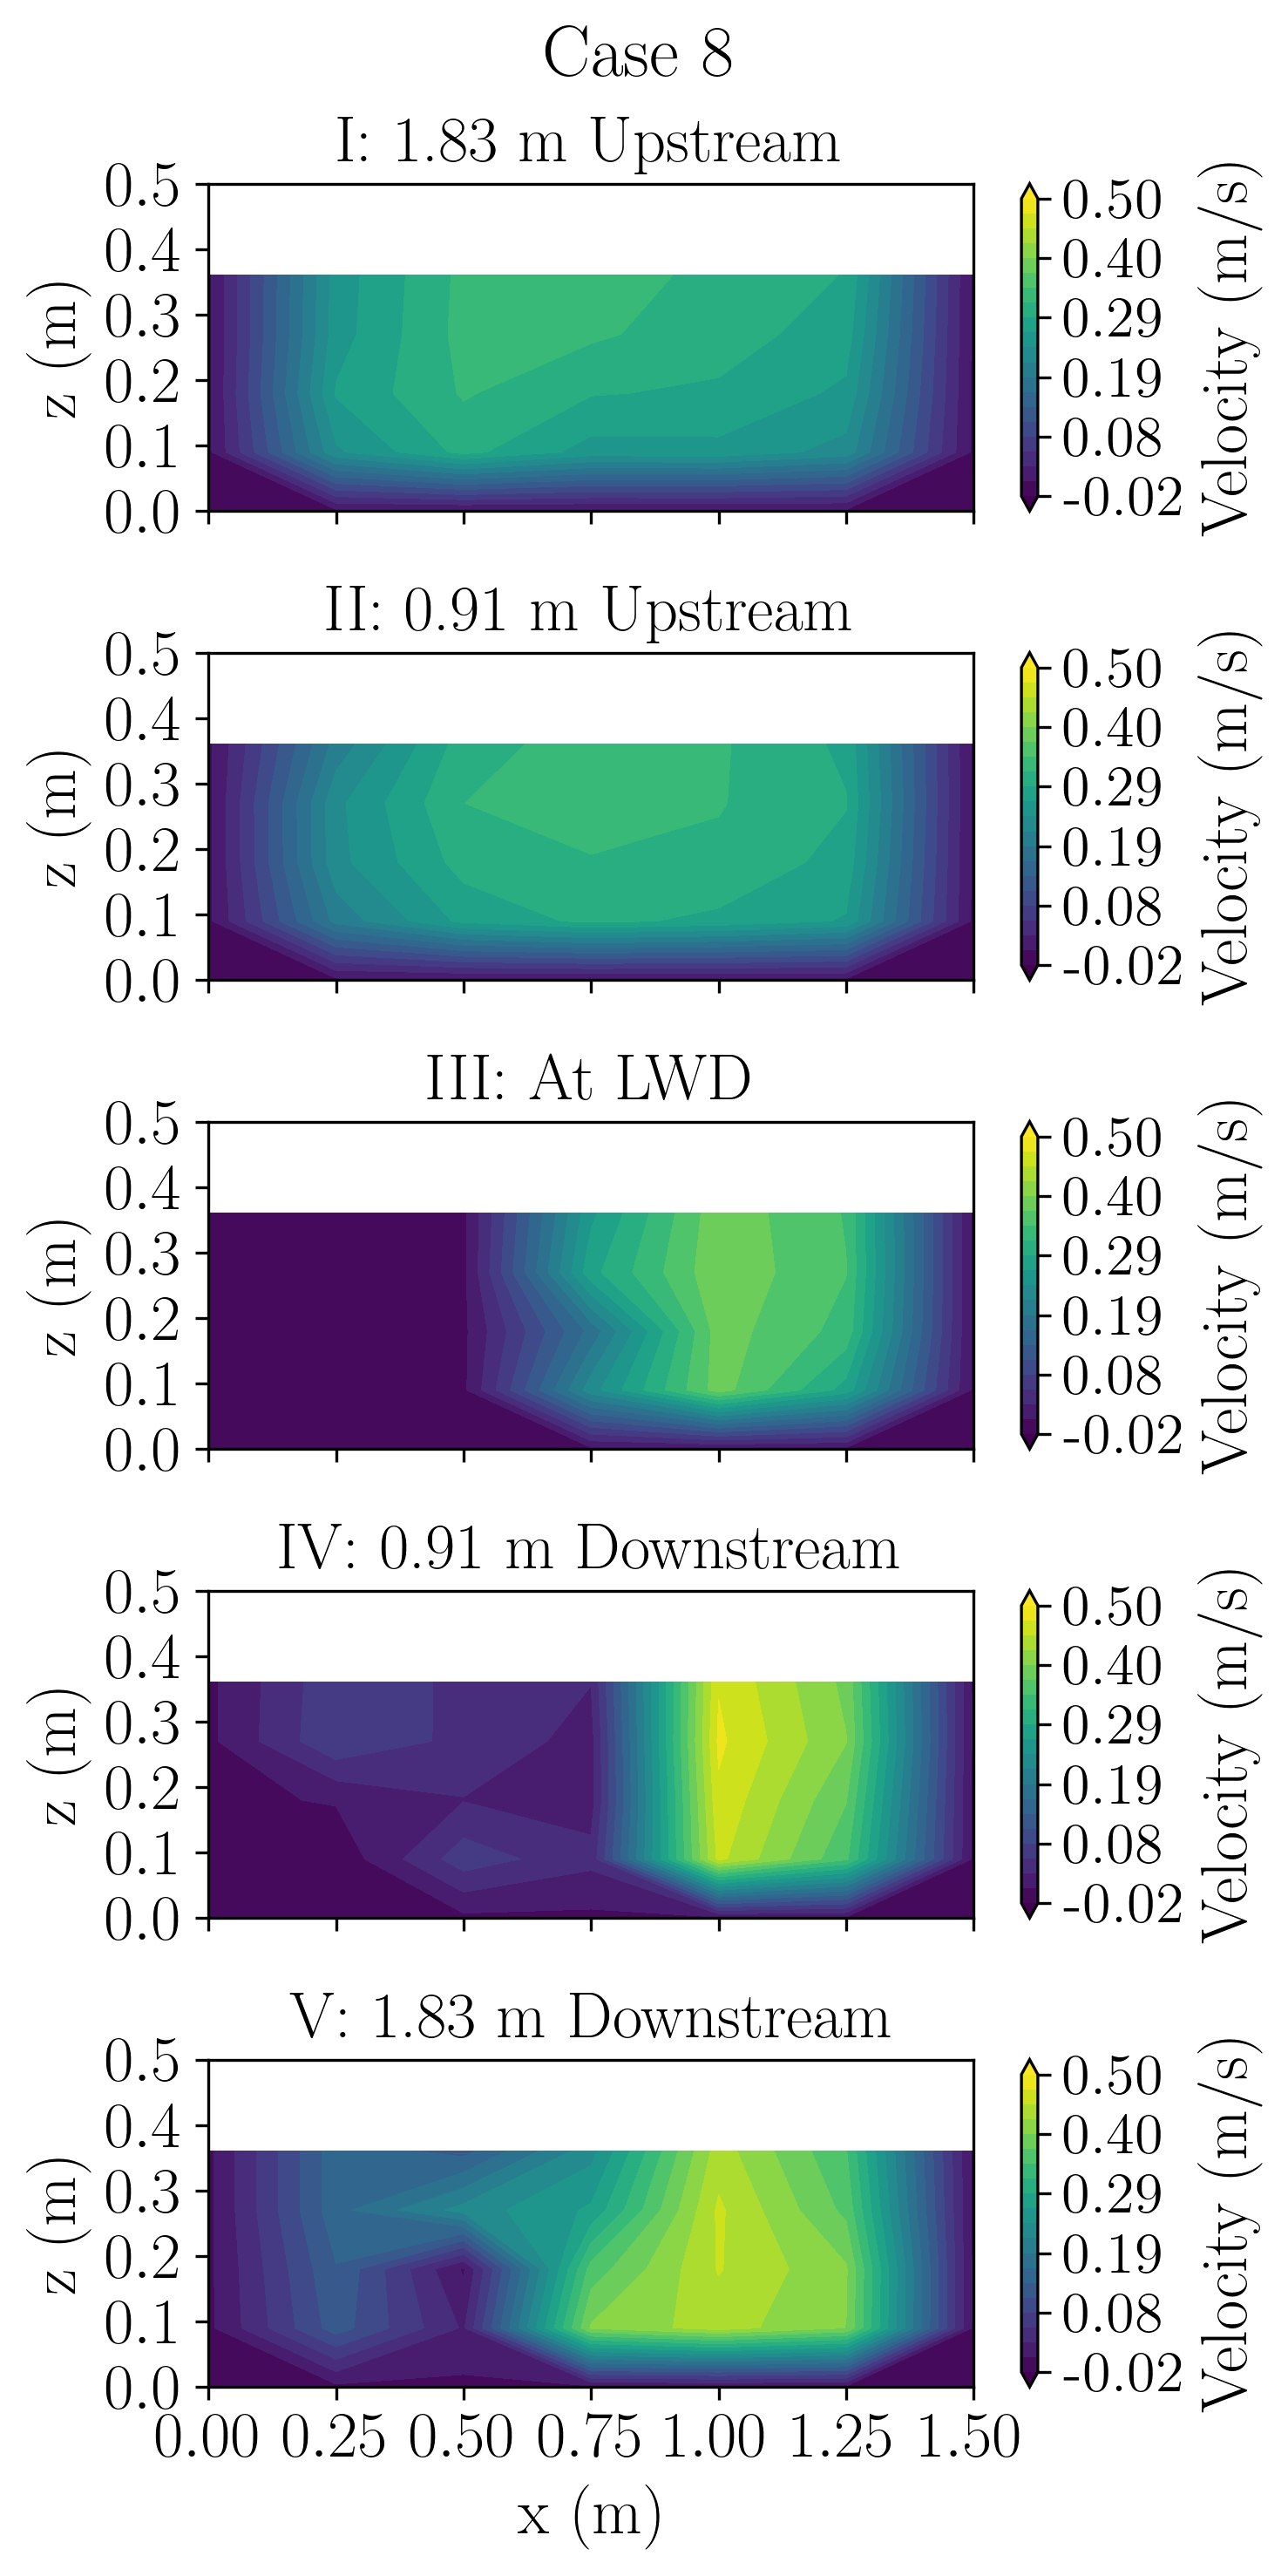
\includegraphics[width=\textwidth]{Case8_velocity_contours.png}
     \end{subfigure}
     \hfill     
     \begin{subfigure}[b]{0.24\textwidth}
         \centering
         \caption{}
         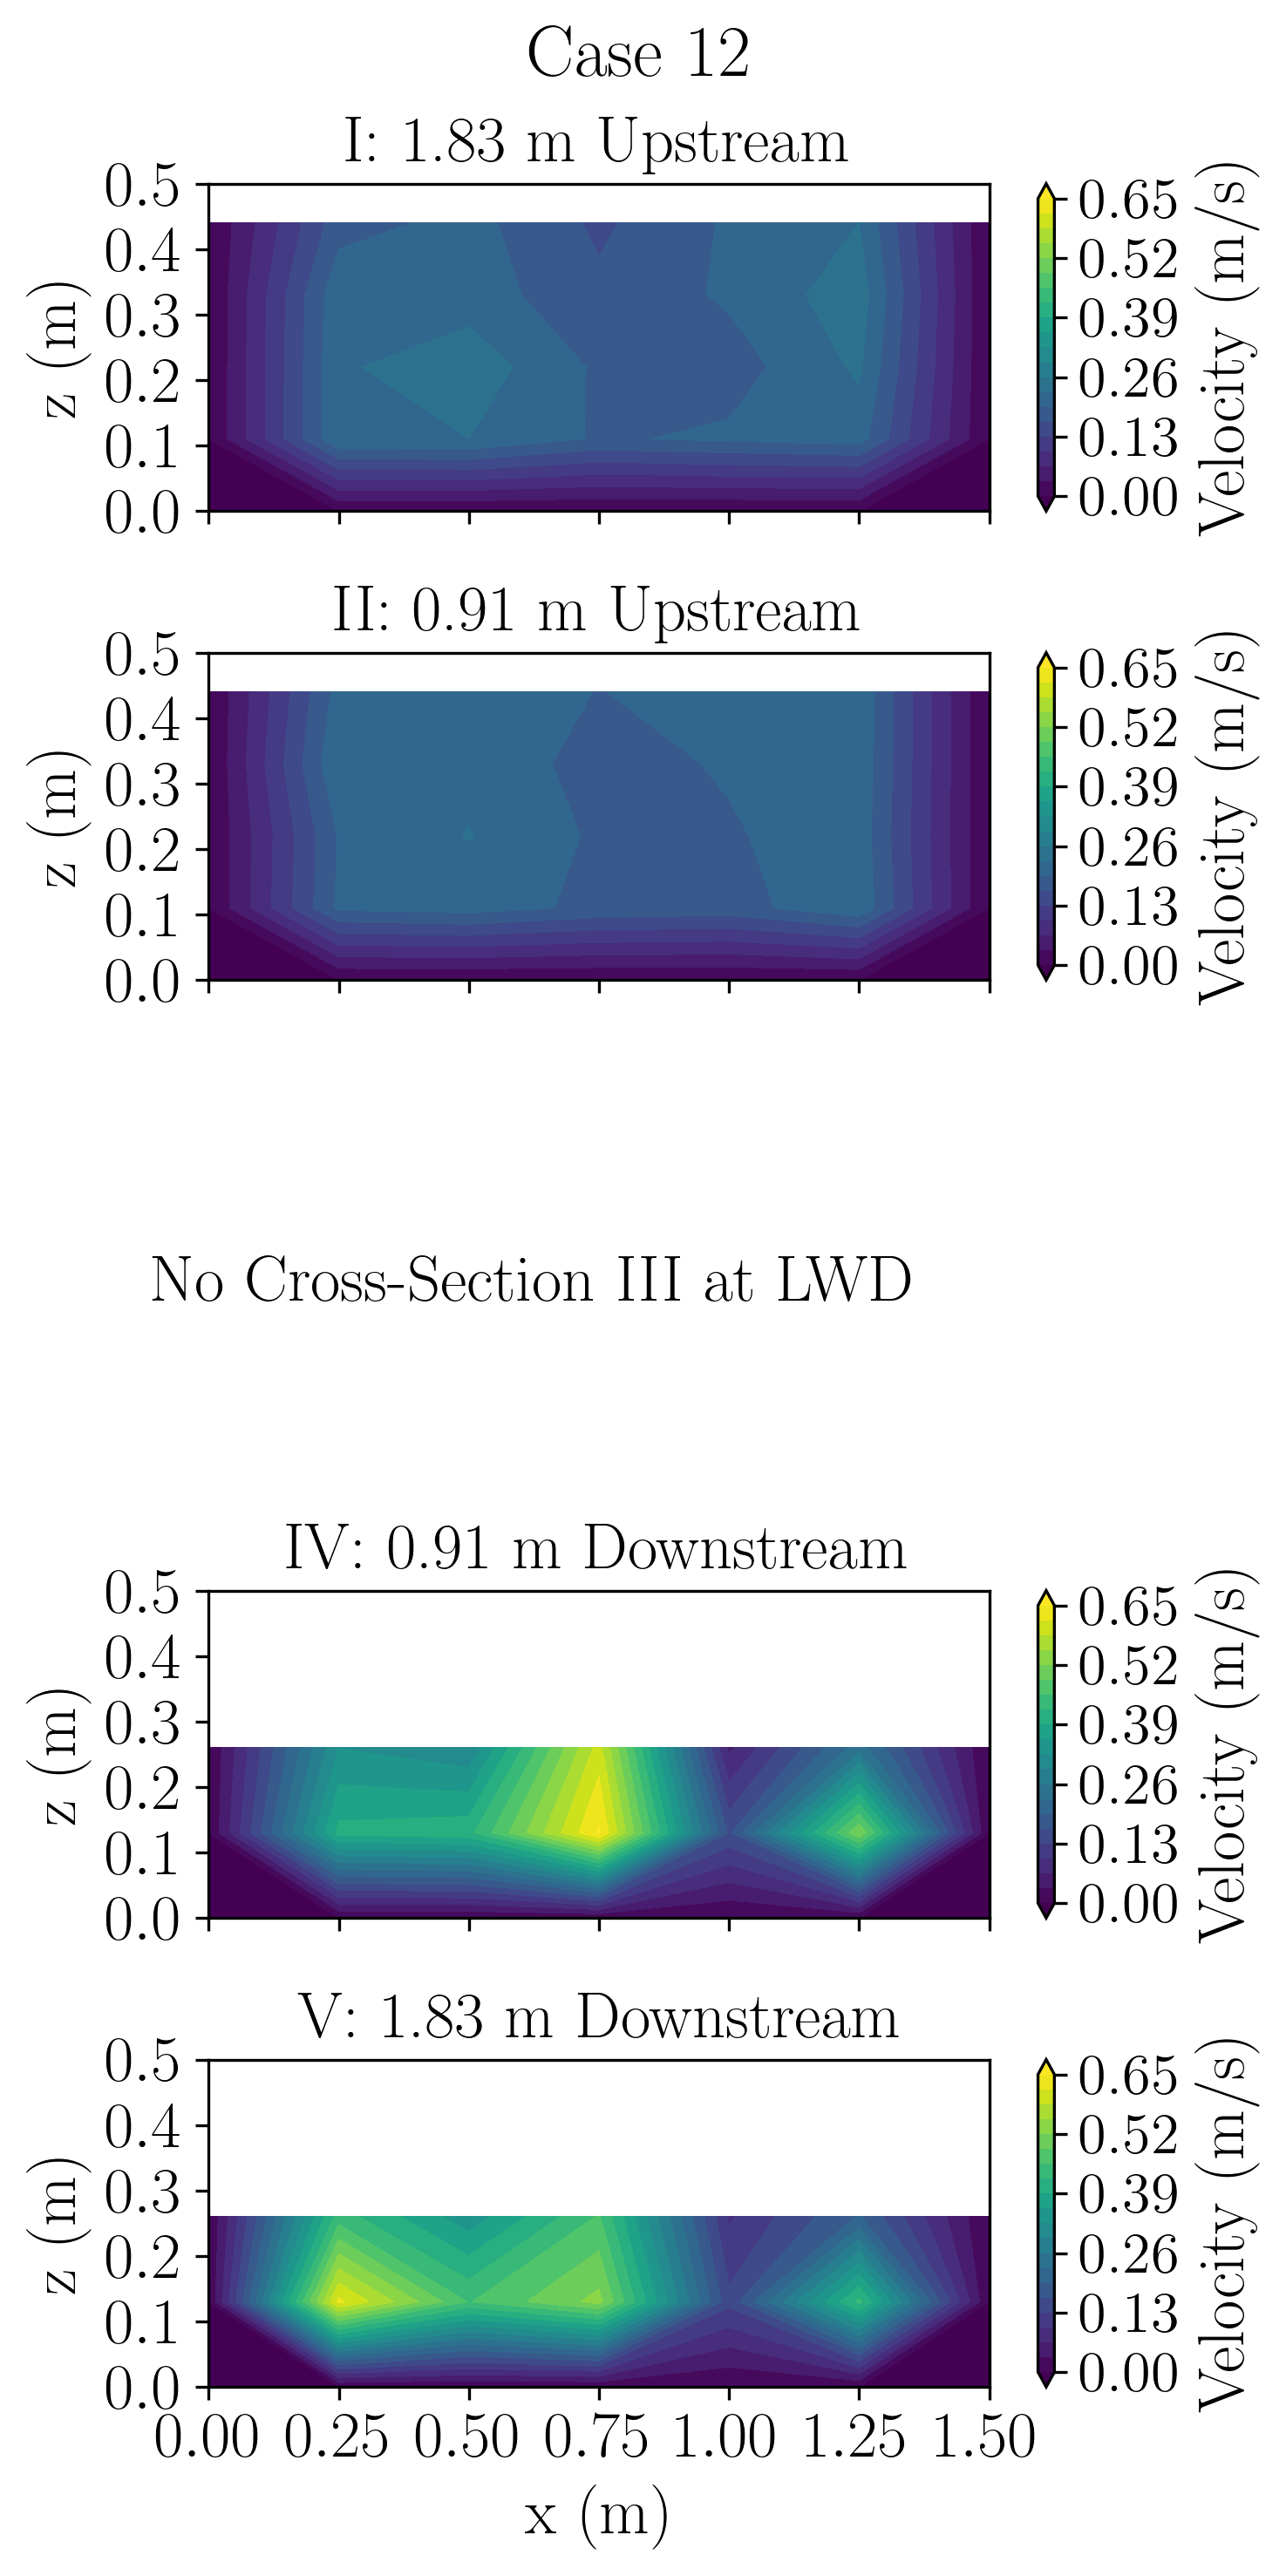
\includegraphics[width=\textwidth]{Case12_velocity_contours.png}
     \end{subfigure}
     \hfill     
     \begin{subfigure}[b]{0.24\textwidth}
         \centering
         \caption{}
         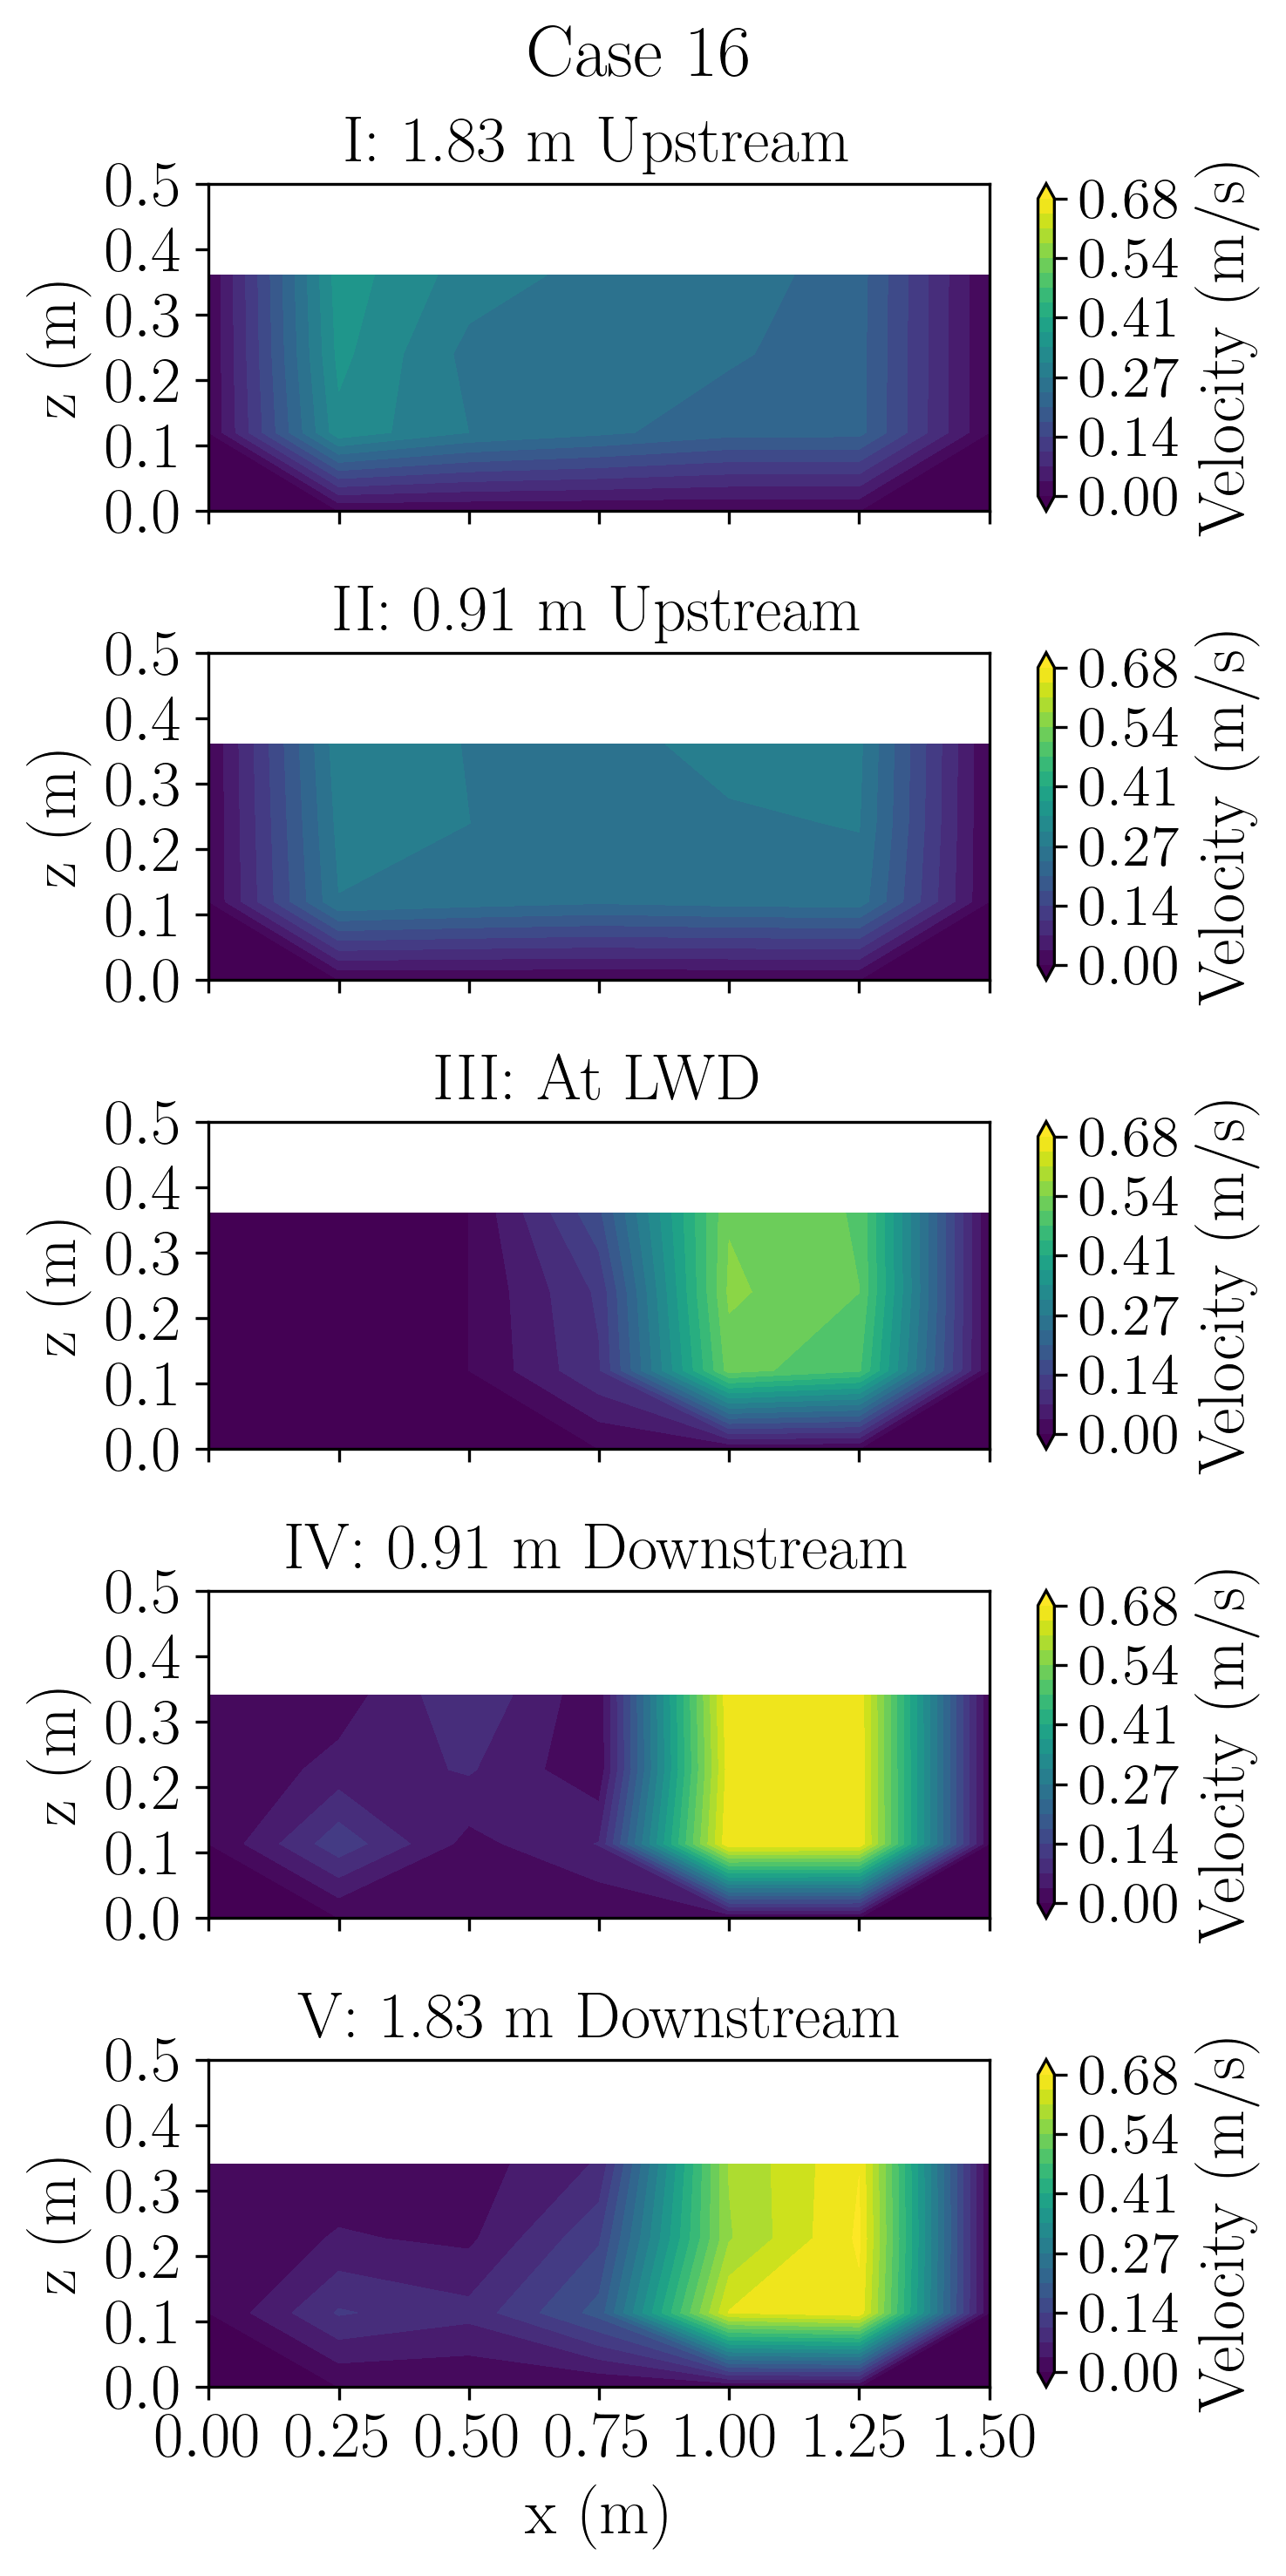
\includegraphics[width=\textwidth]{Case16_velocity_contours.png}
     \end{subfigure}
\end{figure}

\end{document}
